%! TEX program = xelatex
% \documentclass[draft]{beamer}
\documentclass{beamer}

\usepackage{kotex}
% \usepackage{graphicx}
\usepackage{minted}
% \usepackage[export]{adjustbox}
% \usepackage{textcomp}

\vfuzz=30pt

%%%%%%%%%%%%%%%%%%%%%
%  Beamer Settings  %
%%%%%%%%%%%%%%%%%%%%%
\usetheme[numbering=fraction]{metropolis}
\usecolortheme{rose}
\useoutertheme[subsection=false]{miniframes}

\setbeamertemplate{itemize item}[square]
\setbeamertemplate{itemize subitem}[triangle]
\setbeamertemplate{itemize subsubitem}[circle]


%%%%%%%%%%%%%%%%%%%
%  Font Settings  %
%%%%%%%%%%%%%%%%%%%
\usepackage[factor=500]{microtype}

\usefonttheme{professionalfonts} % required for mathspec
\usepackage{mathspec}

\setmathsfont(Digits)[%
  Numbers={Lining, Proportional}
]{Fira Sans}
\setsansfont[%
  BoldFont={Fira Sans SemiBold},
  Numbers={OldStyle}
]{Fira Sans}
\setsanshangulfont{Noto Sans CJK KR}[%
  AutoFakeSlant=0.18,
  FontFace={m}{up}{Font=*}
]

\newfontfamily\NotoSansMonoExtraCondensed{Noto Sans Mono ExtraCondensed}
\RenewDocumentCommand\UrlFont{}{\NotoSansMonoExtraCondensed}
\NewDocumentCommand\textct{m}{{\NotoSansMonoExtraCondensed#1}}

%%%%%%%%%%%%%%%%%%%%%
%  Minted Settings  %
%%%%%%%%%%%%%%%%%%%%%
% \renewcommand\theFancyVerbLine{\textsf{\tiny\arabic{FancyVerbLine}}}
%
\newminted{shell}{
  escapeinside=||,
  % mathescape,
  autogobble,
  % linenos,
  breaklines,
  % numbersep=5pt,
  frame=single,
  fontsize=\footnotesize}
\newmintinline[shverb]{shell}{fontsize=\tiny,escapeinside=||}

%%%%%%%%%%%%%%%%%%%%%%%
% Custom Settings  %
%%%%%%%%%%%%%%%%%%%%%%%
\NewDocumentCommand\tpc{}{\textperiodcentered}
\NewDocumentCommand\tat{}{\textasciitilde}
\NewDocumentCommand\vpad{}{\vspace{1em}}
% \def\tbs{\textbackslash}
%
% \newcommand*{\numberofpages}[1]{%
%   \the\XeTeXpdfpagecount"#1" %
% }


%%%%%%%%%%%%%%%%%%%%%%%
%  Document Settings  %
%%%%%%%%%%%%%%%%%%%%%%%
\title{\TeX{}nical Vim}
\author{이재호}
\institute{서울대학교 전기\tpc{}정보공학부/KTUG}
\date{2020년 2월 15일}

%%%%%%%%%%%%%%
%  Document  %
%%%%%%%%%%%%%%
\begin{document}
% \RenewDocumentCommand\pause{o}{}

\maketitle

%%%%% Hook %%%%%
\begin{frame}[plain]{}
  \begin{tabular}{cccc}
    
\includegraphics[width=0.21\linewidth]{figures/logo-atom} &
    
\includegraphics[width=0.21\linewidth]{figures/logo-bbedit} &
    
\includegraphics[width=0.21\linewidth]{figures/logo-eclipse} &
    
\includegraphics[width=0.21\linewidth]{figures/logo-emacs} \\
    
\includegraphics[width=0.21\linewidth]{figures/logo-gedit} &
    
\includegraphics[width=0.21\linewidth]{figures/logo-notepad} &
    
\includegraphics[width=0.21\linewidth]{figures/logo-notepad++} &
    
\includegraphics[width=0.21\linewidth]{figures/logo-sublime-text-3} \\
    
\includegraphics[width=0.21\linewidth]{figures/logo-texshop} &
    
\includegraphics[width=0.21\linewidth]{figures/logo-texworks} &
    
\includegraphics[width=0.21\linewidth]{figures/logo-vim} &
    
\includegraphics[width=0.21\linewidth]{figures/logo-vscode}
  \end{tabular}
\end{frame}

\begin{frame}[plain]{Editor War (1985\tat{}현재)}
  \centering
\includegraphics[width=0.8\linewidth]{figures/emacs-vs-vim}
\end{frame}

\begin{frame}[plain]{}
  \Large\centering
  그렇다면 어떤 에디터를 쓰는게 제일 좋을까요?\\\pause\vpad
  \large
  여러분의 취향에 맞는 에디터를 쓰세요!\\\pause\vpad
  \alert{한 가지 취향}과 \alert{가능성}을 소개해드리려고 합니다.
\end{frame}

\begin{frame}[plain]{}
  Vim의 가장 큰 무기는 \alert{원하는대로 만들 수 있다는 것}입니다.\\\pause\vpad
  \begin{columns}
    \begin{column}{0.5\linewidth}
      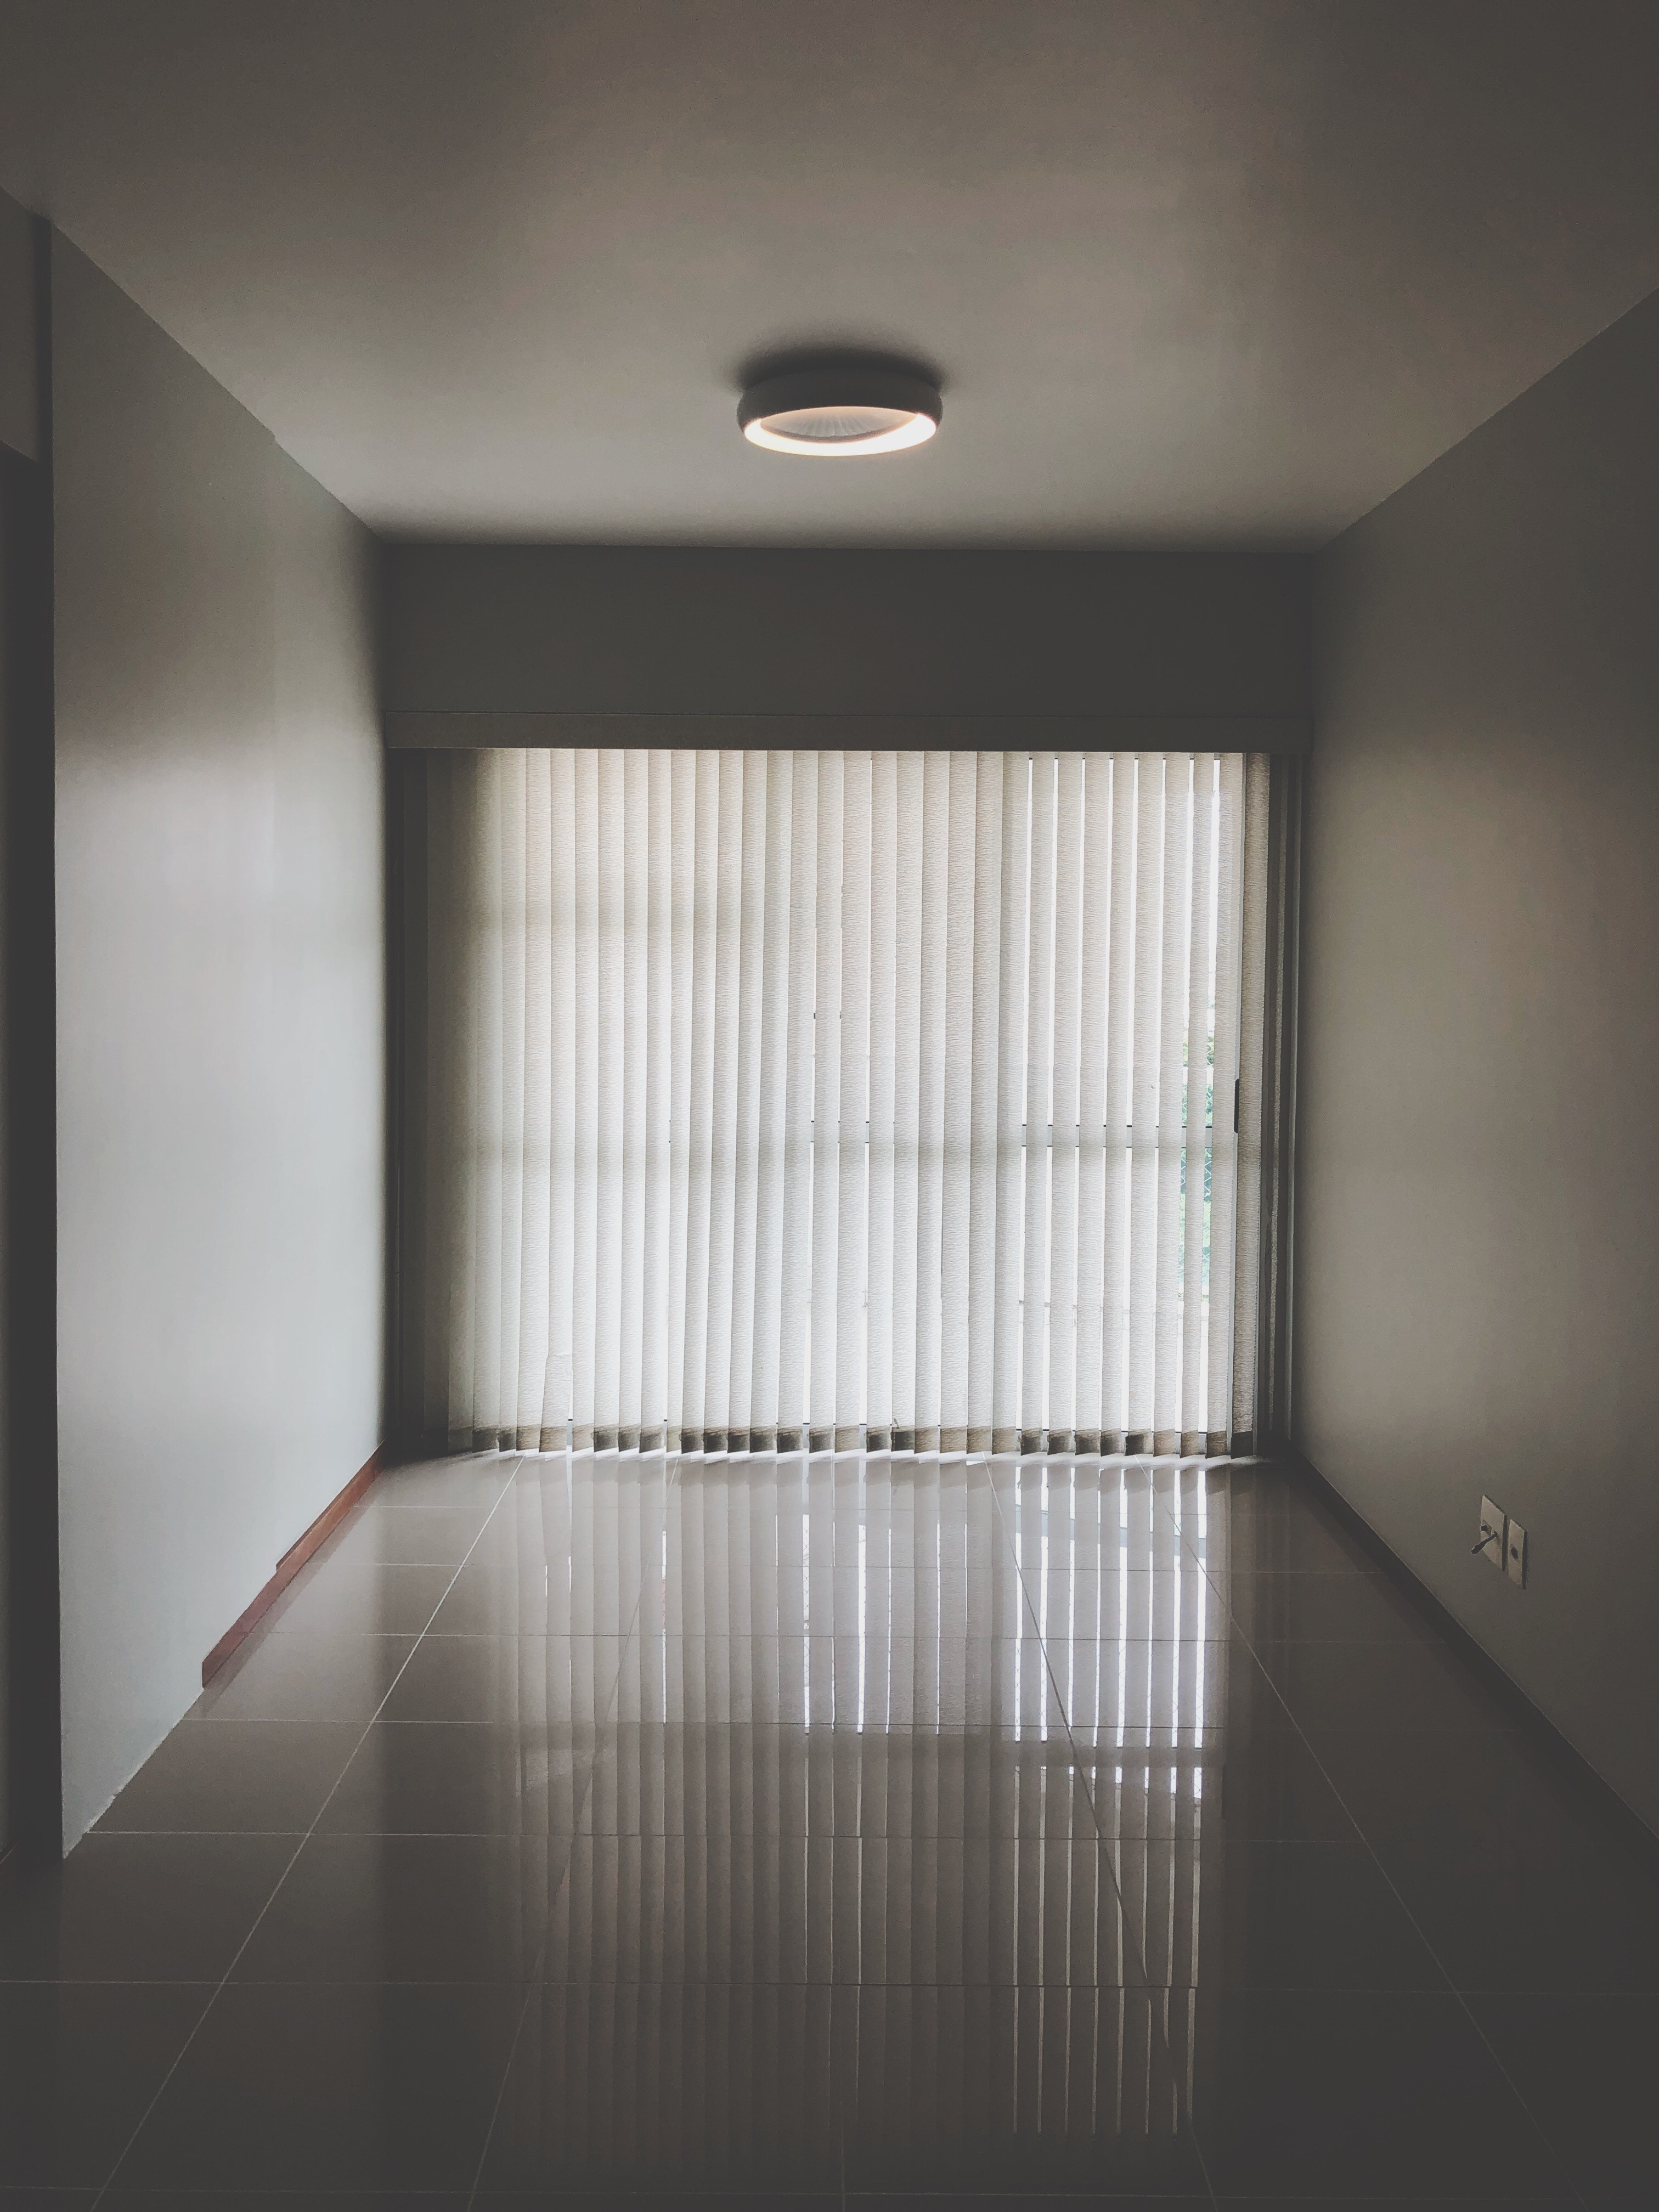
\includegraphics[width=\linewidth]{figures/empty-room}
    \end{column}
    \pause
    \begin{column}{0.5\linewidth}
      \centering
      그러나, 이는 동시에 진입장벽이기도 합니다.\\\pause
      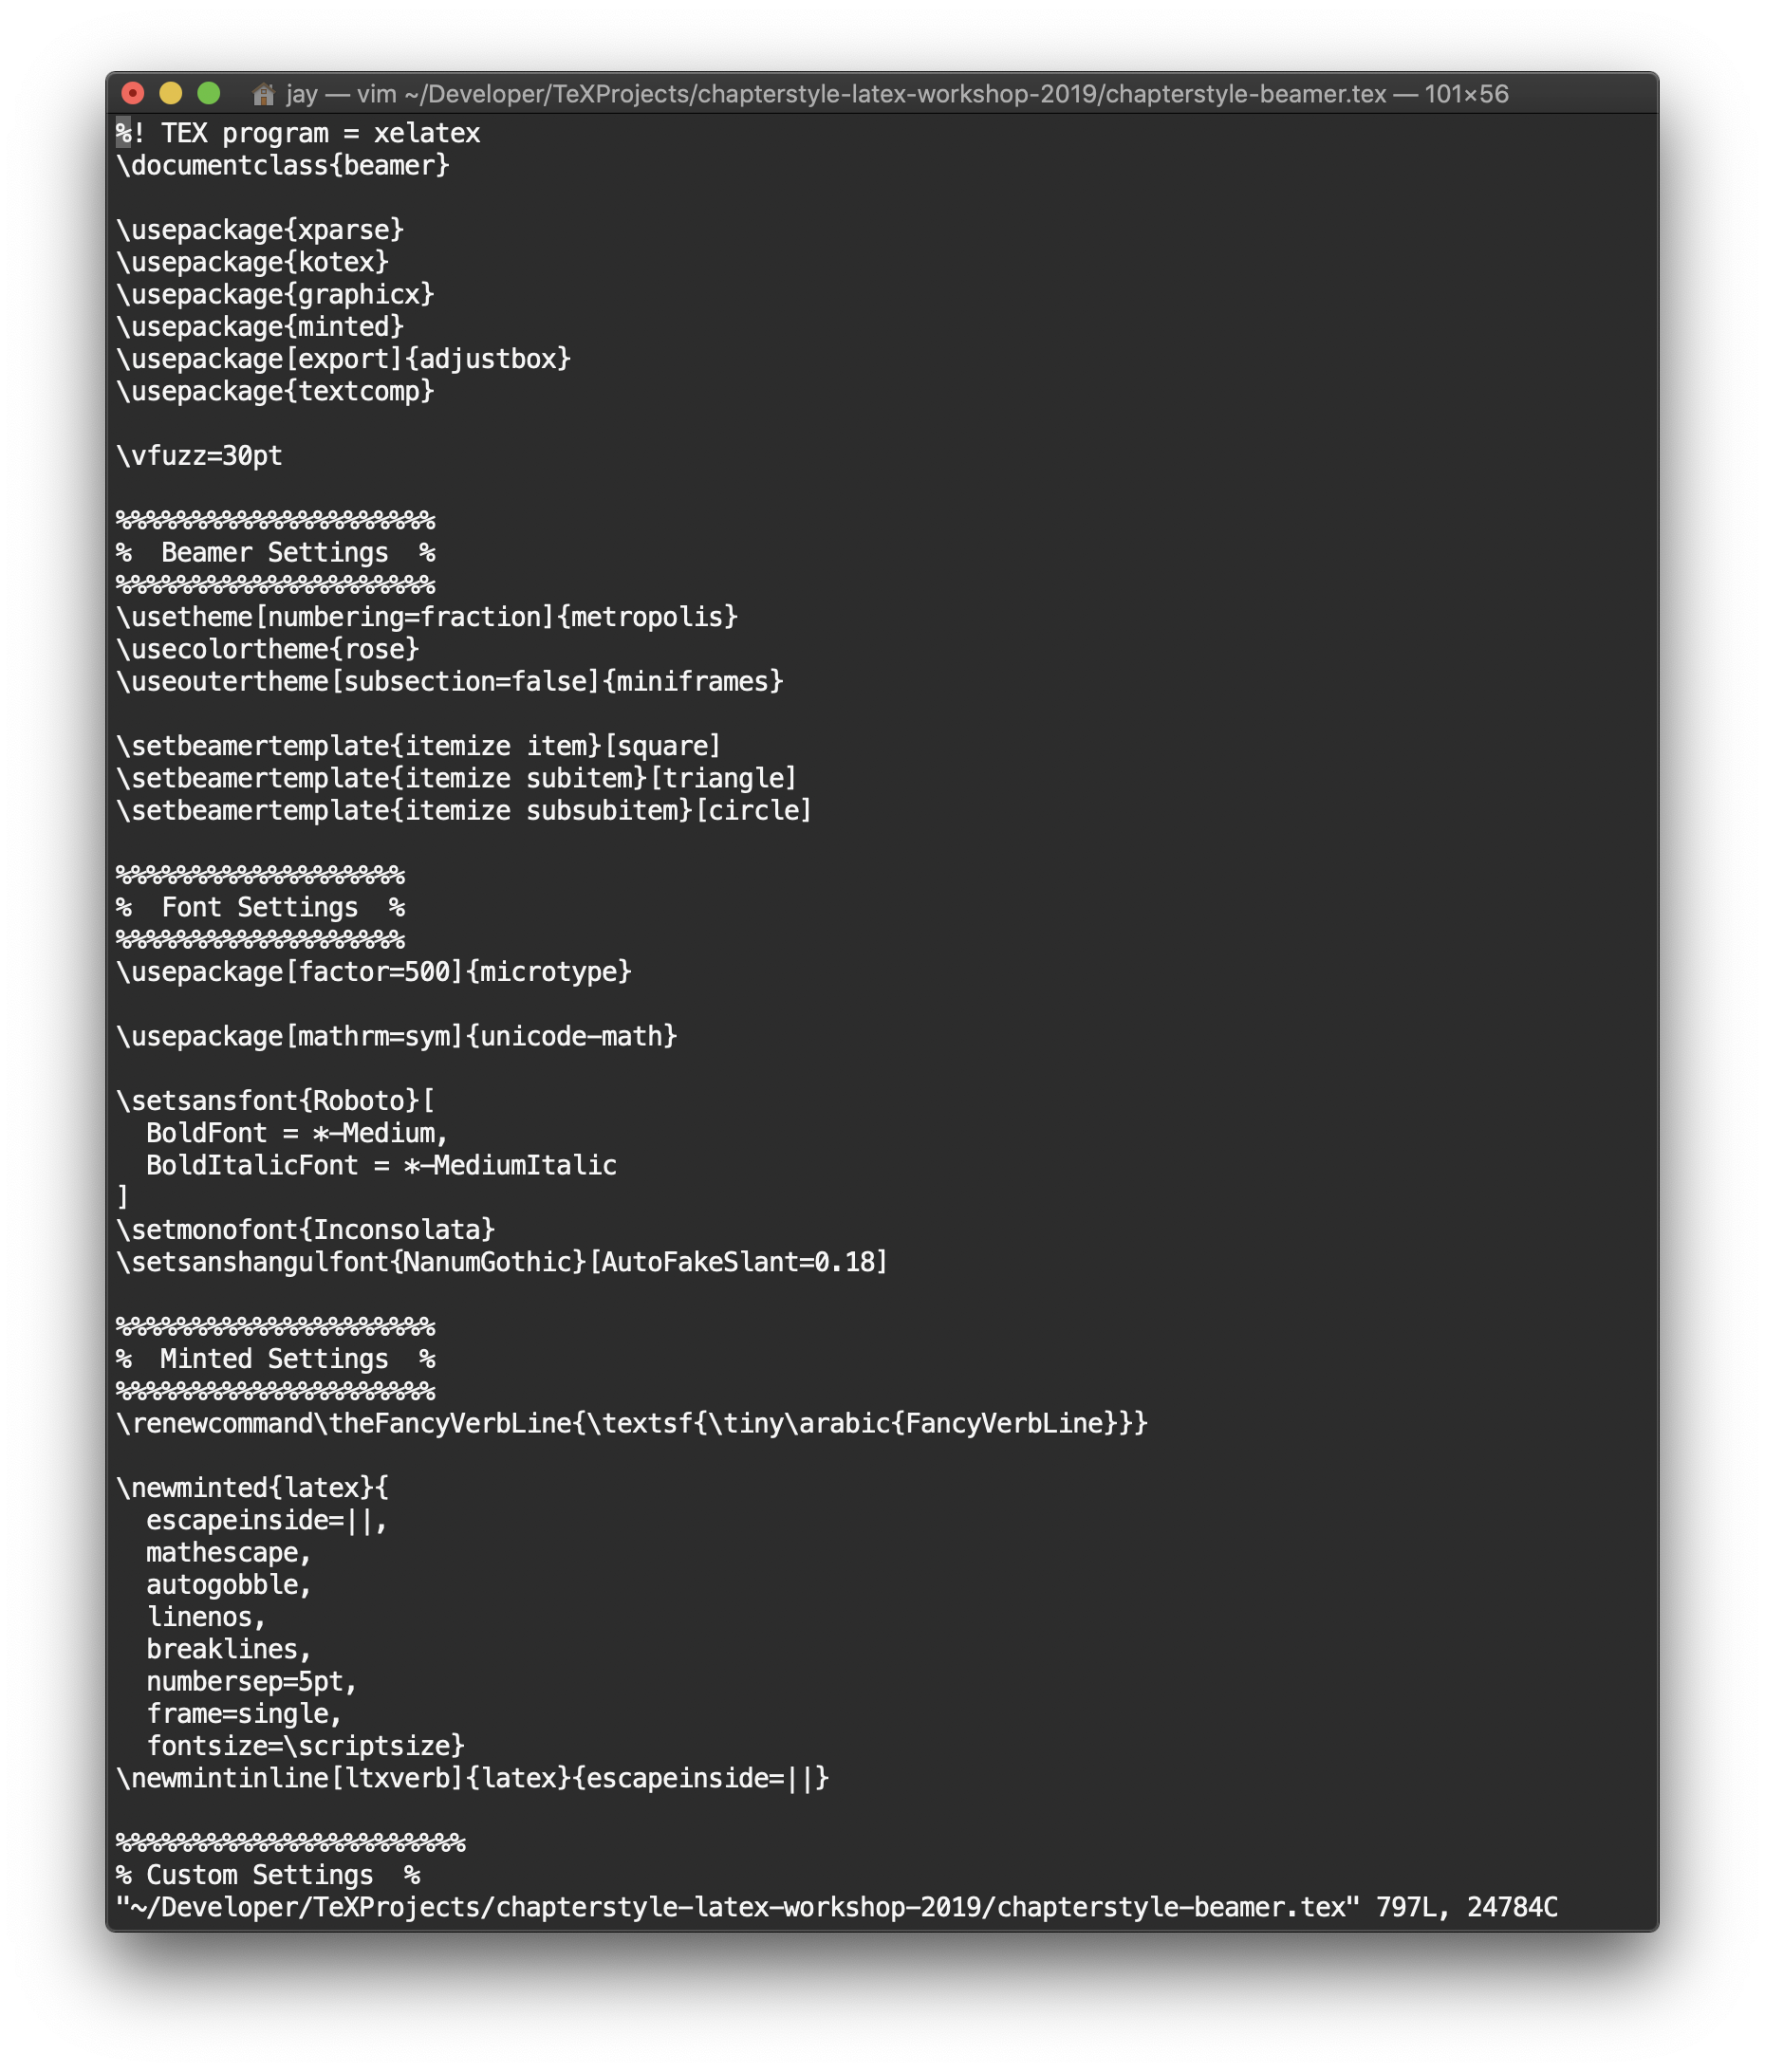
\includegraphics[width=\linewidth]{figures/vanilla-vim}
    \end{column}
  \end{columns}
\end{frame}

\begin{frame}[plain]{가능성}
  \centering\includegraphics[width=\linewidth]{figures/possibility}
\end{frame}

\begin{frame}{본 발표는...}
  \TeX{} 사용자 중
  \begin{enumerate}
    \item Vim에 대해서 들어봤지만 시도하기가 막막하셨던 분들,\pause
    \item Vim을 쓸 줄 알지만 자료가 별로 없어서 \TeX을 Vim에서 쓰지 않았던
      분들,\pause
    \item Vim(혹은 Emacs+AUC\TeX)으로 \TeX을 쓰지만 다른 사람들의 작업 환경이
      궁금하신 분들\pause
  \end{enumerate}
  \vpad
  \centering\alert{Vim으로 \TeX{} 문서를 작성하고 편집하는 효율적인 세팅!}
\end{frame}

\frame[plain]{\tableofcontents}

\section{Why Vim?}

\begin{frame}{첫 번째 관문}
  \TeX{}을 처음 깔았을 때 누구나 마주하는 문제:\\\pause\vpad
  \begin{center}\emph{\TeX{} 문서를 어떤 도구로 만들까?}\end{center}
  \pause\vpad

  가장 기본적인 선택지:
  \begin{itemize}
    \item \TeX{}works (Windows)
    \item \TeX{}Shop (macOS)
  \end{itemize}
\end{frame}

\begin{frame}{Vim이 뭔가요?}
  \pause\centering\alert{\Large Vim은 modal(모달) 에디터입니다.}\pause\vpad
  \begin{itemize}
    \item Normal, Insert, Visual, Command-line 모드
      \begin{itemize}
        \item \textcolor{gray}{와 Ex, Select 모드}
      \end{itemize}
    \pause
    \item \alert{Edit}or라는 이름에 걸맞게, 편집하는 일에 특화
      \begin{itemize}
        \item 반복 작업 및 영역 편집
      \end{itemize}
    \pause
    \item 기본적으로는 터미널에서 사용
      \begin{itemize}
        \item 손은 키보드 위에서만
      \end{itemize}
    \pause
    \item \alert{매우 유연한 설정}
      \begin{itemize}
        \item 그만큼 초기 설정은 매우 적음
      \end{itemize}
  \end{itemize}
\end{frame}

\begin{frame}{왜 X 대신 Vim인가요?}
  \begin{itemize}
    \item X = Electron 계열의 에디터 (Atom, Visual Studio Code)\pause
      \begin{itemize}
        \item 장점
          \begin{itemize}
            \item GUI로 동작하므로 진입장벽이 낮음\pause
            \item \alert{Language server}를 통한 강력한 문법 강조 및 자동
              완성\pause
          \end{itemize}
        \item 단점
          \begin{itemize}
            \item (텍스트 편집을 위해서!) 웹 브라우저(Chromium)의 부하\pause
            \item \alert{Language Server Protocol (LSP)}의 등장\pause
          \end{itemize}
      \end{itemize}
    \item X = Emacs\pause
      \begin{itemize}
        \item 장점
          \begin{itemize}
            \item CLI로 동작함\pause
            \item More than an editor\pause
          \end{itemize}
        \item 단점\pause
          \begin{itemize}
            \item CLI로 동작함
            \item More than an editor
          \end{itemize}
      \end{itemize}
  \end{itemize}
\end{frame}

\begin{frame}{2020년의 Vim}
  \begin{itemize}
    \item User Friendly!\pause
      \begin{itemize}
        \item LSP의 혜택으로 강력한 \alert{문법 강조}, \alert{자동 완성},
          \alert{문법 검증}\pause
          \begin{itemize}
            \item LSP가 너무 무겁다면, 기존 방식의 문법팩 사용 가능
          \end{itemize}
        \item 모든 것이 사용자화 가능\pause
        \item 직관적이고 편한 명령어 (동사 + 명사)\pause
        \item 40년이 넘는 자료와 사용자 그룹\pause
        \item 한 가지 일을 하고, 그것을 잘함
          (\href{https://en.wikipedia.org/wiki/Unix_philosophy}{UNIX Philosophy: Do One Thing and Do It Well})\pause
      \end{itemize}
    \item Developer Friendly!\pause
      \begin{itemize}
        \item Lua를 내장한 Neovim의 등장으로 Lua로 스크립팅이 가능해짐
          \textcolor{gray}{(Lua\TeX?)}\pause
        \item 커뮤니티 기반 (무엇이 Vim이고 Neovim일까요?)\\
          \vspace{5pt}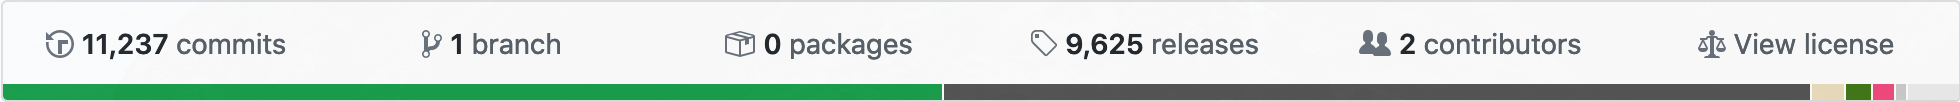
\includegraphics[width=\linewidth]{figures/guess-what-1}\\
          \vspace{2pt}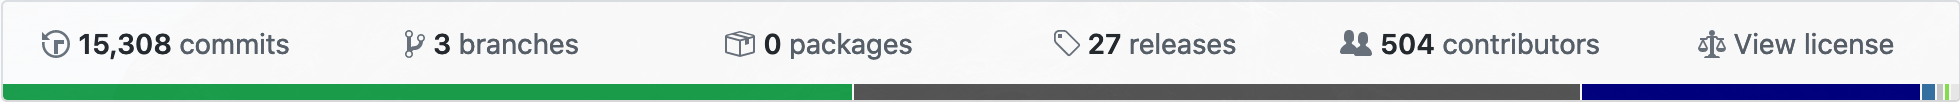
\includegraphics[width=\linewidth]{figures/guess-what-2}
      \end{itemize}
  \end{itemize}
\end{frame}

\begin{frame}
  
\includegraphics[width=\linewidth]{figures/logo-neovim}
\end{frame}

\section{Vim Setup}

\begin{frame}[fragile]{\TeX{}nical Vim 설정 (for macOS)}
  macOS용 package manager인 \href{https://brew.sh/}{Homebrew} 사용
  \begin{enumerate}
    \item \url{https://brew.sh/}를 참고하여 \href{https://brew.sh/}{Homebrew}를 설치합니다.
    \item \href{https://iterm2.com/}{iTerm2},
      \href{https://www.tug.org/mactex/}{Mac\TeX},
      \href{https://skim-app.sourceforge.io/}{Skim}을 설치합니다.
      \begin{shellcode}
        brew tap homebrew/cask
        brew cask install iterm2 mactex skim
      \end{shellcode}
      \begin{description}
        \item[iTerm2] Color scheme, \alert{option key mapping}, powerline
          glyphs, ...
        \item[Mac\TeX] \TeX{}Live의 macOS용 재배포
        \item[Skim] Sync\TeX{} support, automatic refresh, ...
      \end{description}
  \end{enumerate}
  %https://www.sumatrapdfreader.org/free-pdf-reader.html
  %https://github.com/microsoft/terminal
\end{frame}

\begin{frame}[fragile]{\TeX{}nical Vim 설정 (for Windows)}
  Windows용 package manager인 \href{https://chocolatey.org/}{Chocolatey} 사용
  \begin{enumerate}
    \item \url{https://chocolatey.org/install}을 참고하여
      \href{https://chocolatey.org/}{Chocolatey}를 설치합니다. (명령어가 너무
      길어 링크로 대체)
    \item \href{http://wiki.ktug.org/wiki/wiki.php}{KTUG Wiki}를 참고하여,
      \href{http://mirror.navercorp.com/CTAN/systems/texlive/tlnet/install-tl.zip}{install-tl.zip}의
      압축을 풀고 \textct{install-tl-windows.bat}을 실행하여 설치합니다.
    \item 
      \begin{shellcode}
        choco install microsoft-windows-terminal neovim sumatrapdf
      \end{shellcode}
      \begin{description}
        \item[Windows Terminal] Color scheme (that supports iTerm themes!),
          \alert{option key mapping}, powerline glyphs, ...
        \item[SumatraPDF] Sync\TeX{} support, automatic refresh, ...
      \end{description}
  \end{enumerate}
\end{frame}

\section{Hello, Vim!}

\section{\TeX{}nical Vim}

\begin{frame}[standout]
  감사합니다.
\end{frame}

\begin{frame}{부록}
  발표 자료: \url{https://github.com/Zeta611/texnical-vim-kts-conf-2020}

  Neovim 설정: \url{https://github.com/Zeta611/dotfiles}

  \centering
\includegraphics[width=0.35\linewidth]{figures/how-great-vim-is}
\end{frame}
\end{document}
